\section{Appendix}
\label{sec:Appendix}

%\paragraph{3D representation of the First stage}\mbox{}\\
\begin{figure}[hbt!]
    \centering
    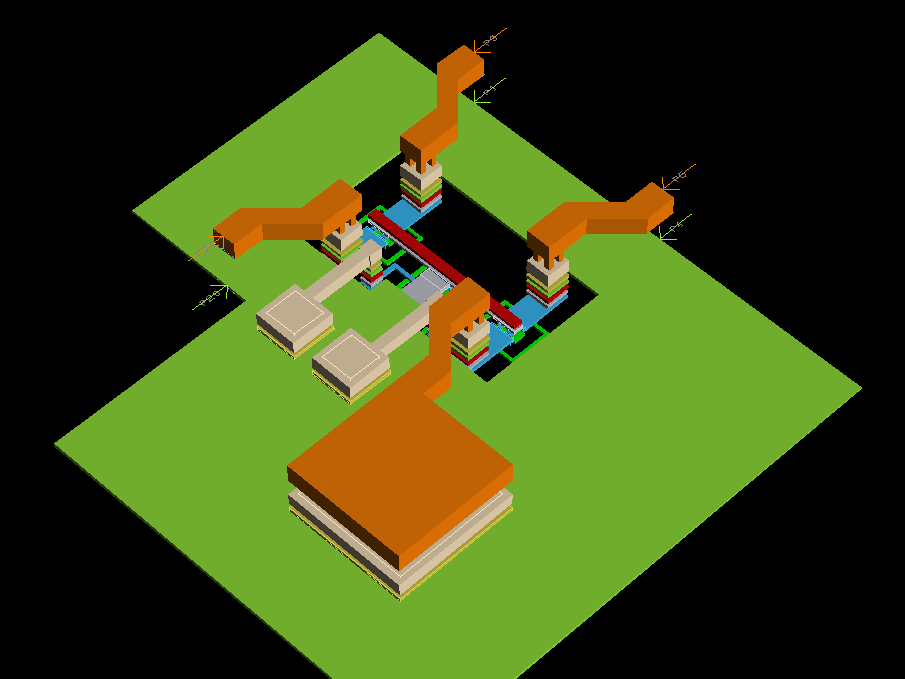
\includegraphics[width=0.65\linewidth]{Design_figures/Layout/Screenshot 2025-10-13 120118.png}
    \caption{layout of the first stage in the 3D view}
    \label{fig:3Dlayoutview}
\end{figure}
%
%\paragraph{First stag}\mbox{}\\
\begin{figure}[hbt!]
    \centering
    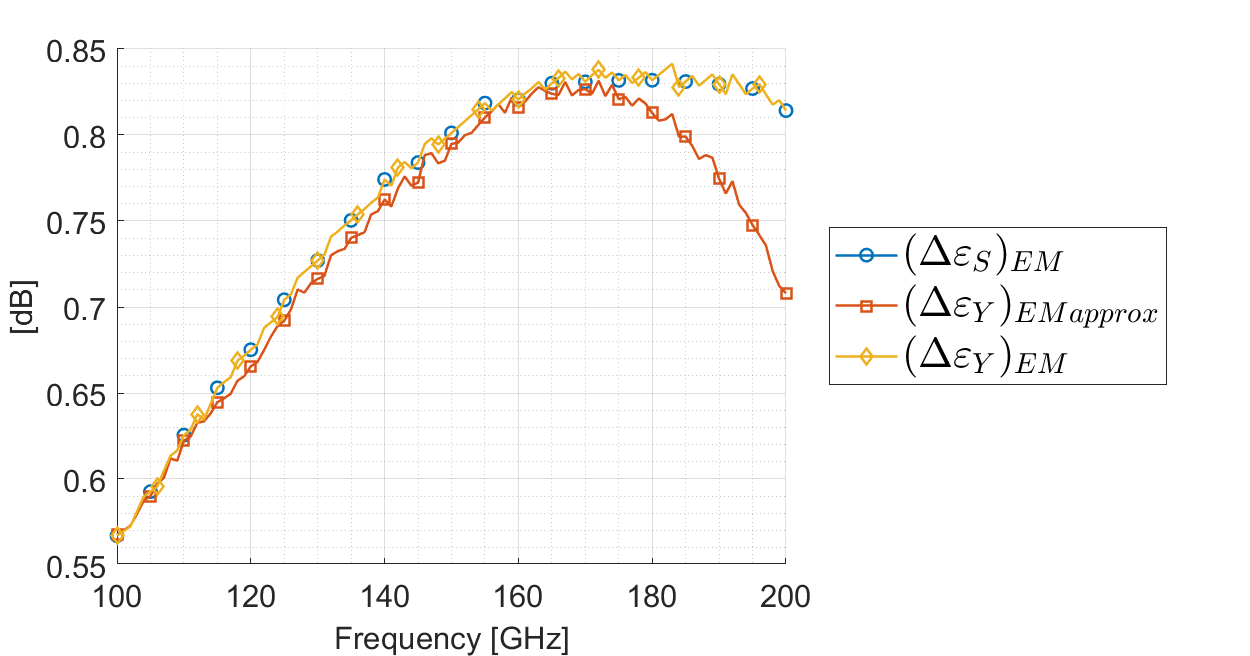
\includegraphics[width=0.75\linewidth]{Design_figures/Layout/ComparisonMeasurements/DiffBalun1Z_ExtractPar_C1C2fixed_S_MaxGain_ComparisonEmBalun_DiffAmp.png}
 \caption{Simulation for amplitude imbalance using different parameters: S \eqref{eq:DiffGainBalanceSports}, Approximated Y \eqref{eq:DiffGainBalanceYportsApprox} and non approximated Y parameters \eqref{eq:DiffGainBalanceYportsComplete}}
    \label{fig:DiffAmpS_vsY}
\end{figure}

%\paragraph{Simulation and comparison of the third-stage inductors}\mbox{}\\
\begin{figure}[htbp!]
\noindent
\begin{minipage}[t]{0.39\linewidth}
    \centering
    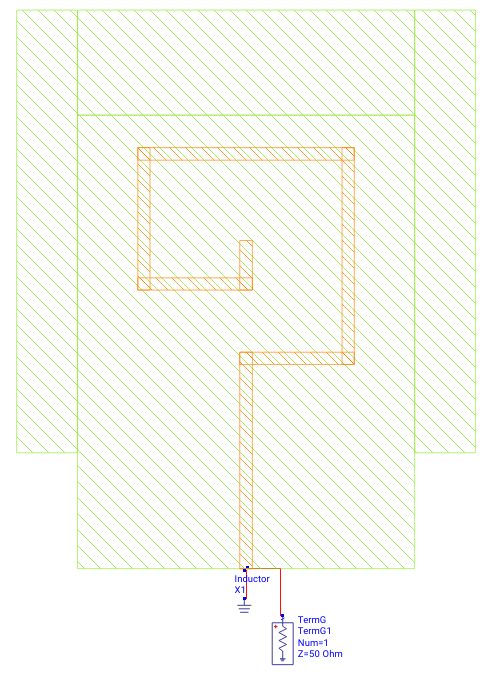
\includegraphics[width=\linewidth]{Design_figures/Layout/LayoutComponents/SchematicComponents/LayoutSpiral_InductorComponent.png}
    \captionof*{figure}{(a)}
\end{minipage}
\hspace{0.01\textwidth}
\begin{minipage}[t]{0.59\linewidth}
    \centering
    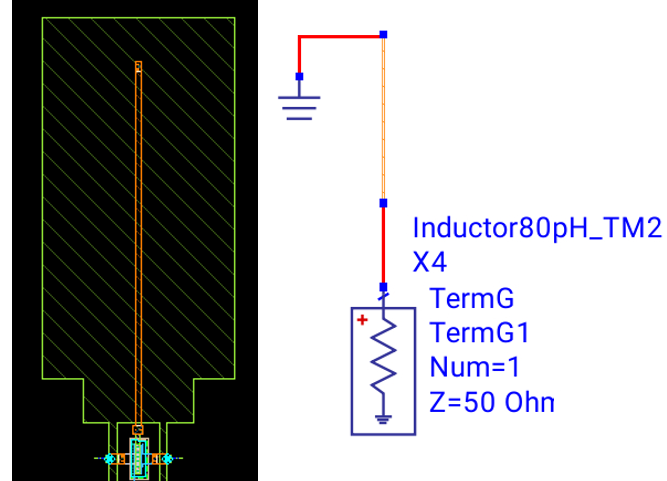
\includegraphics[width=\linewidth]{Design_figures/Layout/LayoutComponents/SchematicComponents/LayoutLine_InductorComponent.png}
    \captionof*{figure}{(b)}
\end{minipage}
 \caption{layout of inductor line topologies tested in the CB amplifier: (a) the spiral inductor chosen for the final layout and (b) straight transmission line}
    \label{fig:LayoutSpiral_vs_Line_indcutorComponent}
\end{figure}
%%%%
%%%%%
\begin{figure}[htbp!]
\noindent
\begin{minipage}[t]{0.49\linewidth}
    \centering
    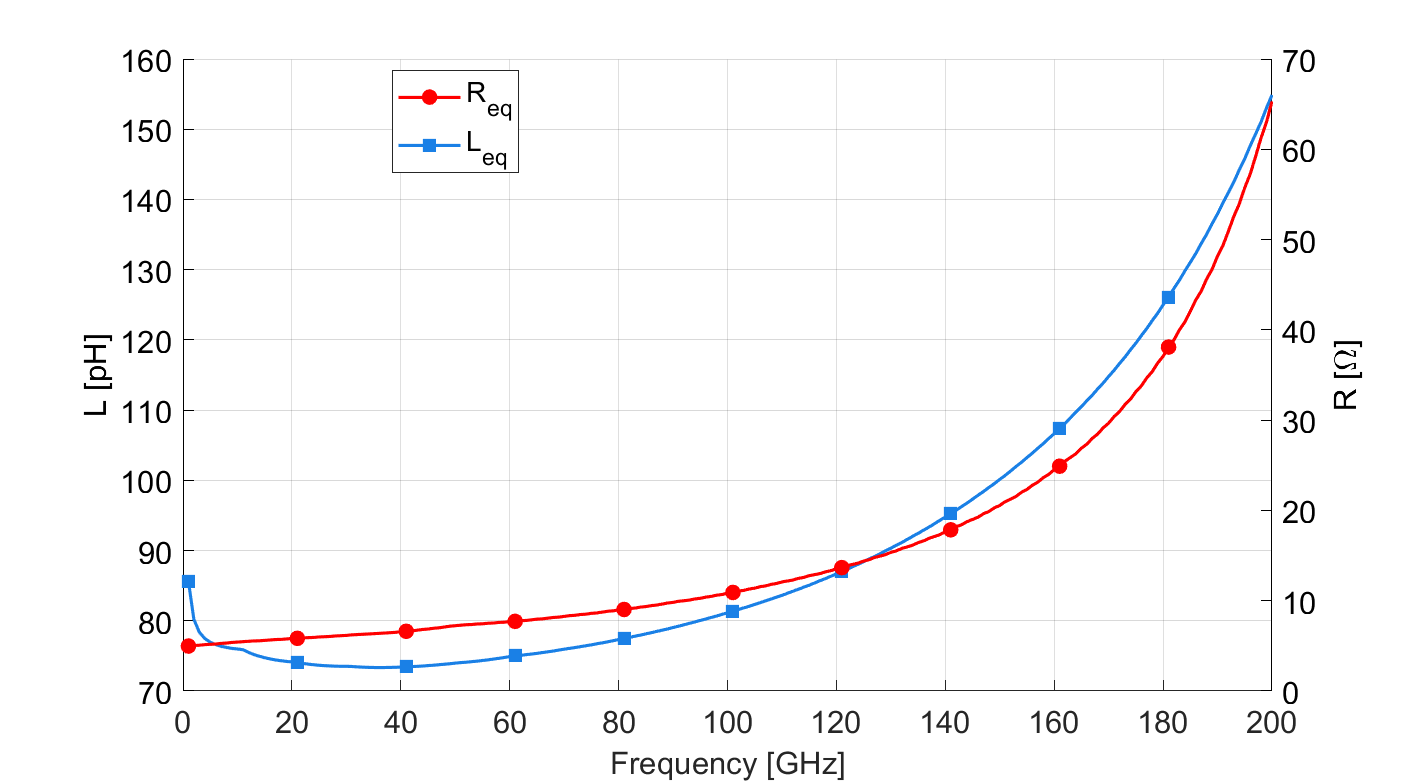
\includegraphics[width=\linewidth]{Design_figures/Layout/LayoutComponents/MeasurementsComponents/LayoutSpiral_InductorComponent_measureL&R.png}
    \captionof*{figure}{(a)}
\end{minipage}
\hspace{0.01\textwidth}
\begin{minipage}[t]{0.49\linewidth}
    \centering
    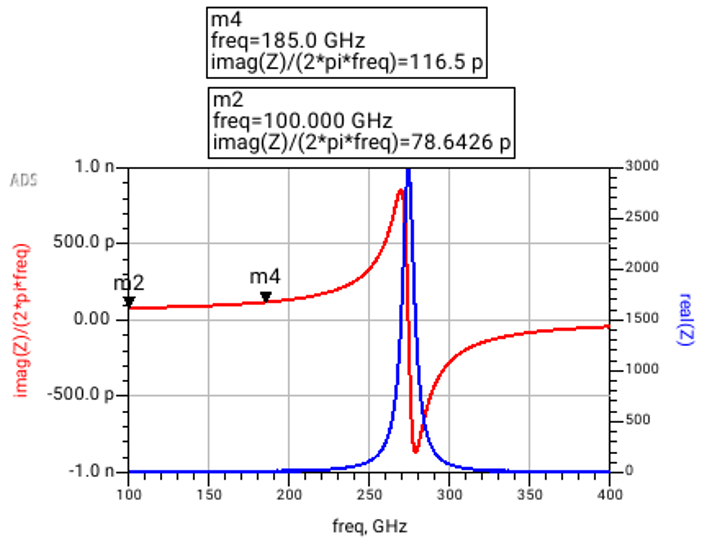
\includegraphics[width=\linewidth]{Design_figures/Layout/LayoutComponents/MeasurementsComponents/LayoutLine_InductorComponent_measureL&R.png}
    \captionof*{figure}{(b)}
\end{minipage}
 \caption{Simulations of inductance and resistance: (a) the spiral inductor simulated in ADS and extracted from the CSV file and (b) the straight-line inductor simulated in ADS}
    \label{fig:LayoutSpiral_vs_Line_indcutorComponent_measureL&R}
\end{figure}

%%%%


%%%%%
\begin{figure}[hbt!]
\noindent
\begin{minipage}[t]{0.49\linewidth}
    \centering
    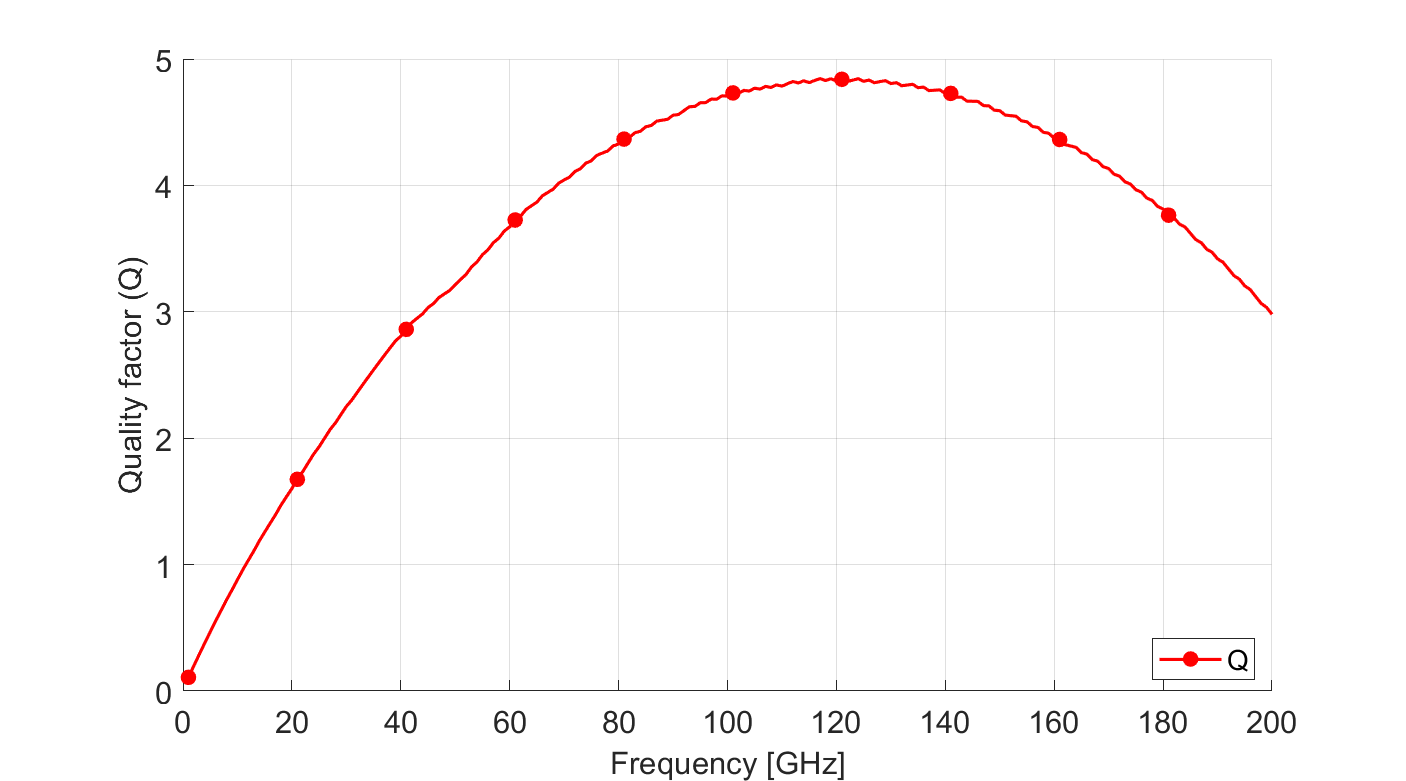
\includegraphics[width=\linewidth]{Design_figures/Layout/LayoutComponents/MeasurementsComponents/LayoutSpiral_InductorComponent_measureQ.png}
    \captionof*{figure}{(a)}
\end{minipage}
\hspace{0.01\textwidth}
\begin{minipage}[t]{0.49\linewidth}
    \centering
    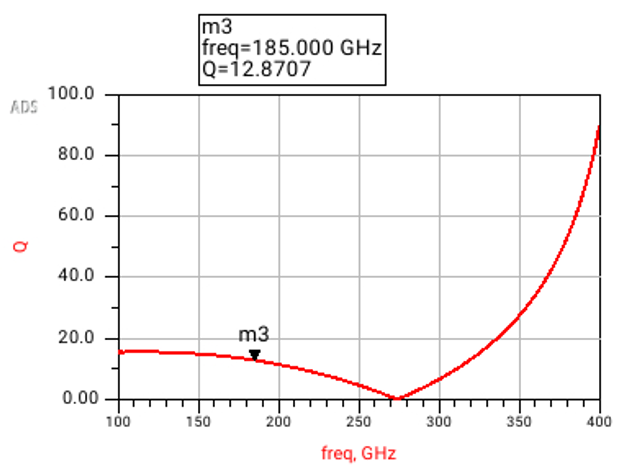
\includegraphics[width=\linewidth]{Design_figures/Layout/LayoutComponents/MeasurementsComponents/LayoutLine_InductorComponent_measureQ.png}
    \captionof*{figure}{(b)}
\end{minipage}
 \caption{Simulations of quality factor: (a) the spiral inductor simulated in ADS and extracted from the CSV and (b) the straight-line inductor from an older simulation figure.}
    \label{fig:LayoutSpiral_vs_Line_indcutorComponent_measureQ}
\end{figure}
%

%\paragraph{Third stage layout with ideal middle components}\mbox{}
\begin{figure}[hbt!]
    \centering
    \begin{minipage}[]{0.25\linewidth}
        \centering
        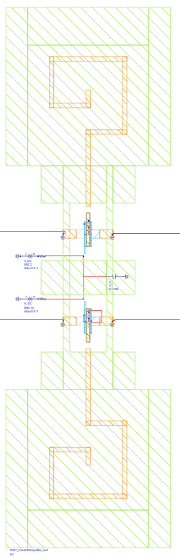
\includegraphics[width=\linewidth]{Design_figures/Schematics/CBamplifierSweepCapacitor.PNG}
        \\ (a)
        \label{fig:firststage_amplitude_imbalance}
    \end{minipage}
    \hfill
    \begin{minipage}[]{0.55\linewidth}
        \centering
        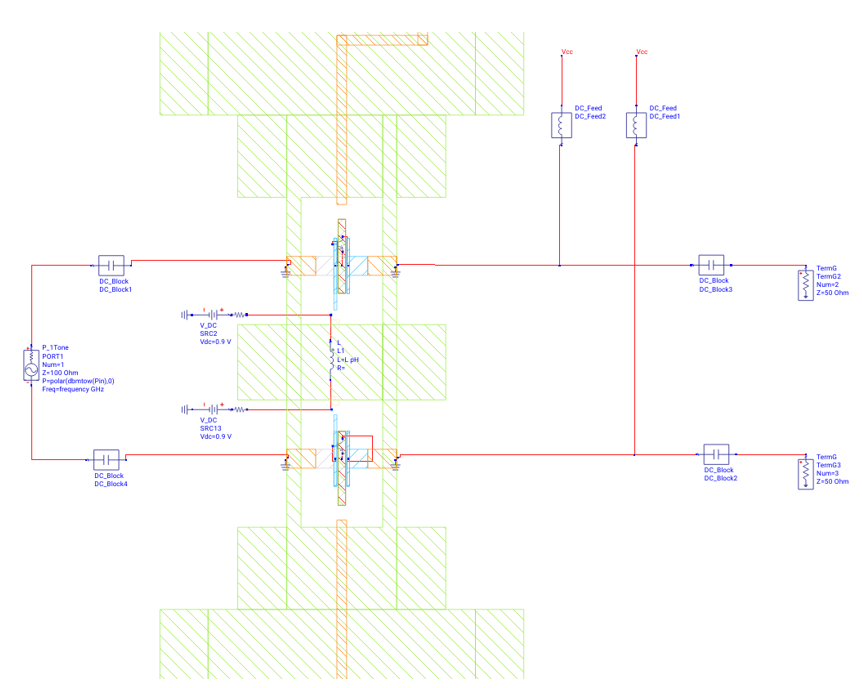
\includegraphics[width=\linewidth]{Design_figures/Schematics/CBamplifierSweepInductor.png}
        \\ (b)
        \label{fig:firststage_phase_imbalance}
    \end{minipage}
    \caption{Schematic of the CB amplifier with differential input during sweeps of the middle-ideal component: (a) capacitor sweep and (b) inductor sweep.}
    \label{fig:cb_amplifier_sweeps}
\end{figure}
\begin{figure}[hbt!]
    \centering
    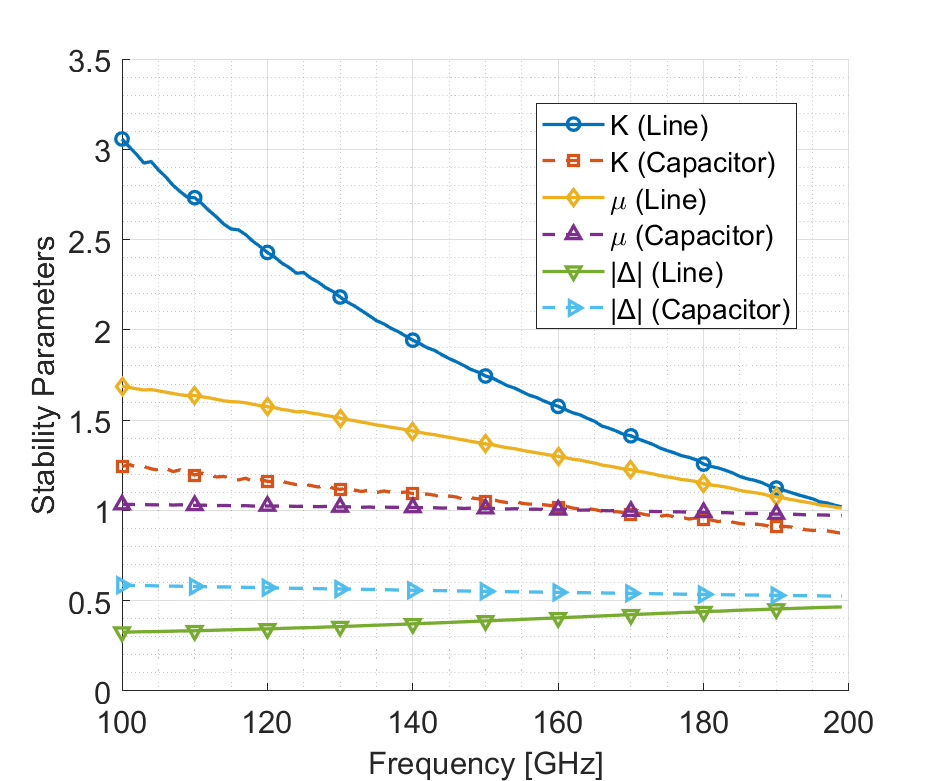
\includegraphics[width=0.52\linewidth]{Design_figures/Measurements/ThirdStage/processEM_ThirdStage_CompareMidCap_VS_inductorLineStability_Metrics_Comparison.png}
    \caption{Simulation and comparisons for the stability parameters of the symmetric third stage amplifier with EM shunt capacitor versus the Metal1 transmission lines between the bases.}
\label{fig:processEM_ThirdStage_CompareMidCap_VS_inductorLineStability_Metrics_Comparison.png}
\end{figure}
%
\noindent
%\paragraph{Stability behavior comparison of the EM third stages}\mbox{}
\begin{figure}[hbt!]
    \centering
    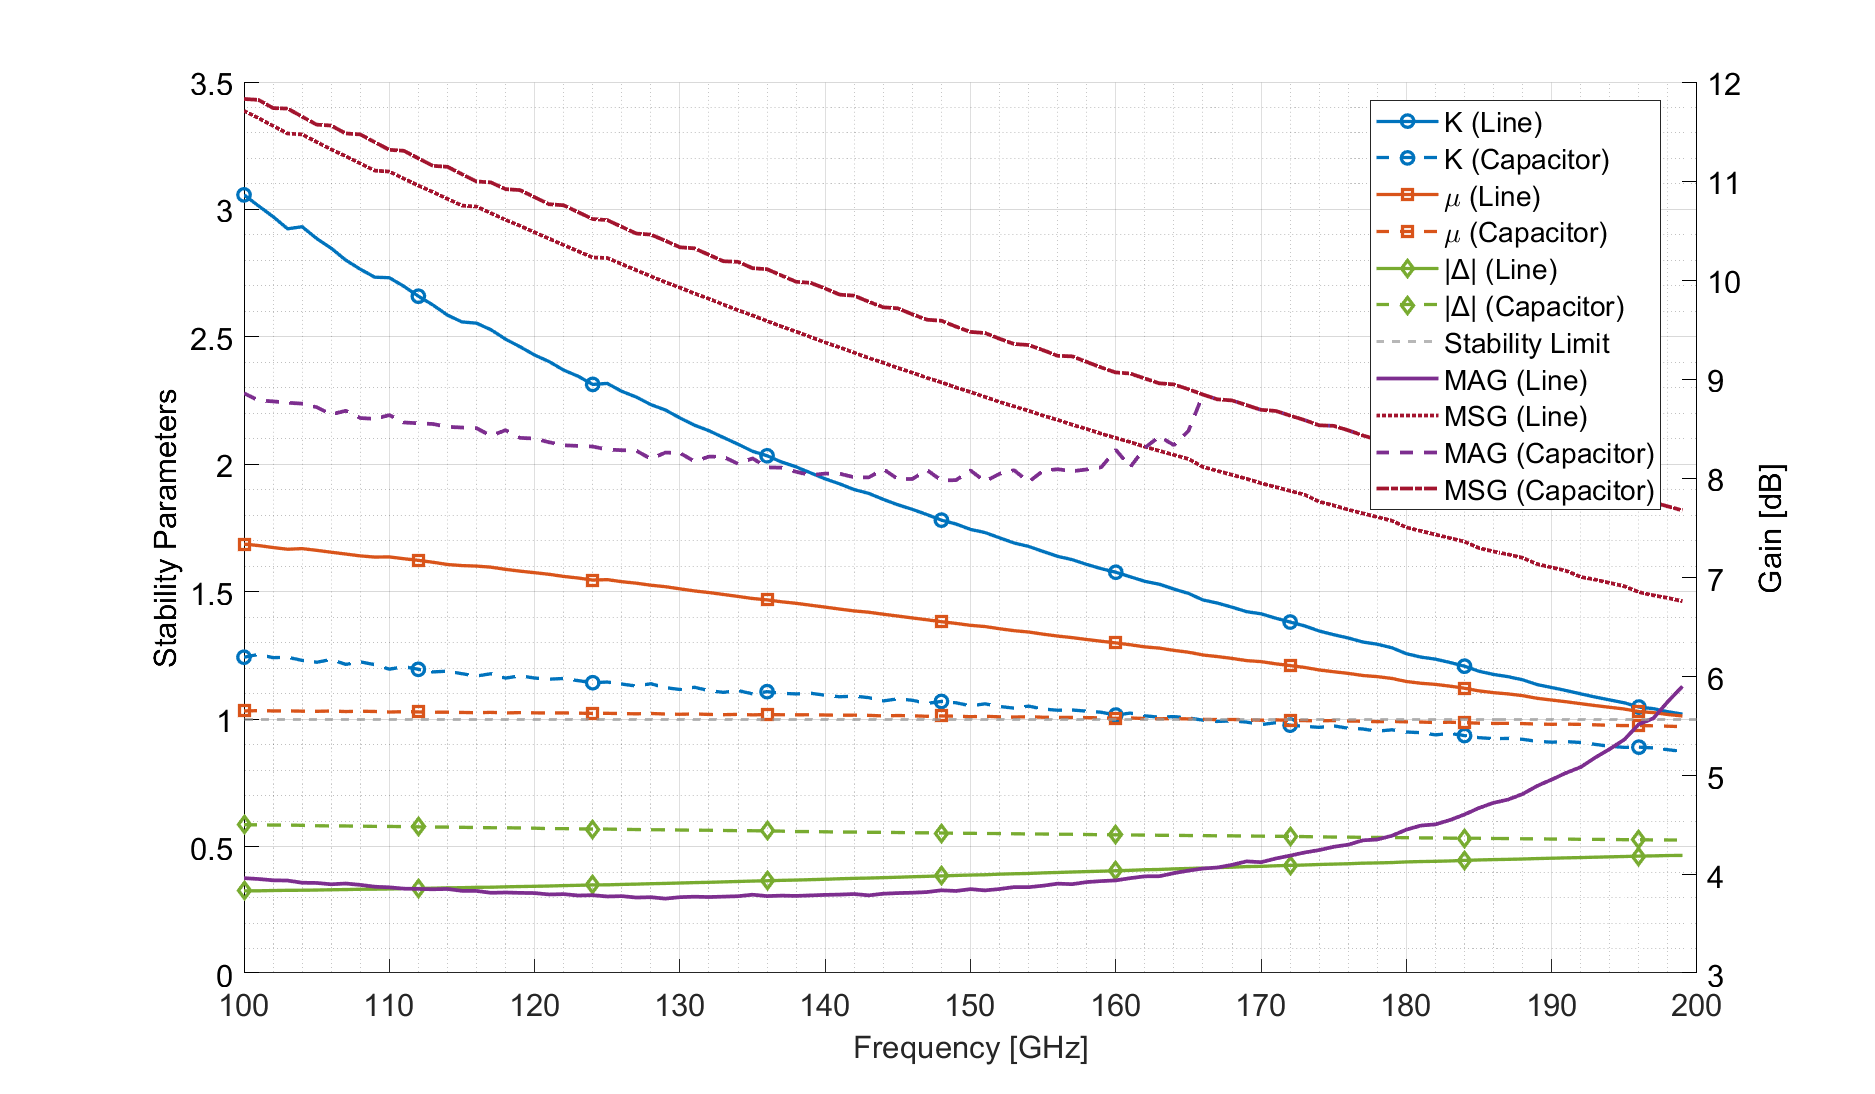
\includegraphics[width=0.85\linewidth]{Design_figures/Measurements/ThirdStage/processEM_ThirdStage_CompareMidCap_VS_inductorLineStability_and_Gain_Comparison.png}
    \caption{Simulation and comparisons for the MaxGains and for the stability parameters in the symmetric third stage amplifier with EM shunt capacitor versus the Metal1 transmission lines between the bases.}
\label{fig:processEM_ThirdStage_CompareMidCap_VS_inductorLineStability_and_Gain_Comparison.png}
\end{figure}

%\paragraph{Simulation results of component values}\mbox{}\\
\begin{figure}[hbt!]
\noindent
\begin{minipage}[t]{0.39\linewidth}
    \centering
    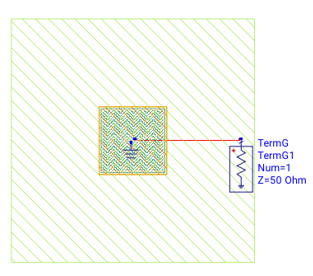
\includegraphics[width=\linewidth]{Design_figures/Layout/LayoutComponents/SchematicComponents/EM_ShuntCapacitor_Layout.png}
    \captionof*{figure}{(a)}
\end{minipage}
\hspace{0.01\textwidth}
\begin{minipage}[t]{0.59\linewidth}
    \centering
    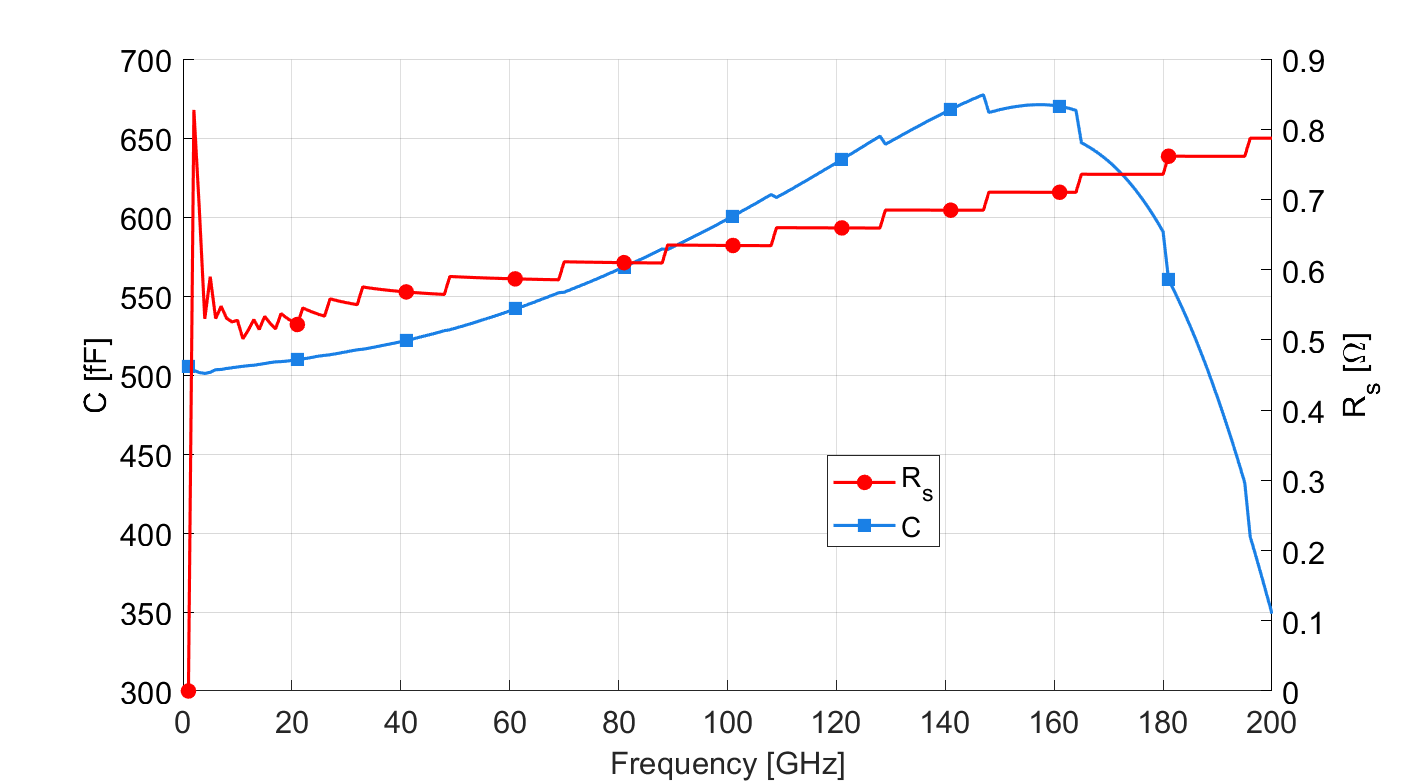
\includegraphics[width=\linewidth]{Design_figures/Layout/LayoutComponents/MeasurementsComponents/LayoutCapacitor_measureC_Rs.png}
    \captionof*{figure}{(b)}
\end{minipage}
 \caption{(a) Schematic of the EM simulated capacitor $C_1$ and (b) impedance simulated in ADS and extracted from the CSV file in MATLAB.}
    \label{fig:Layout_ShuntCapacitor}
\end{figure}

\begin{comment}
    \begin{figure}
    \centering
    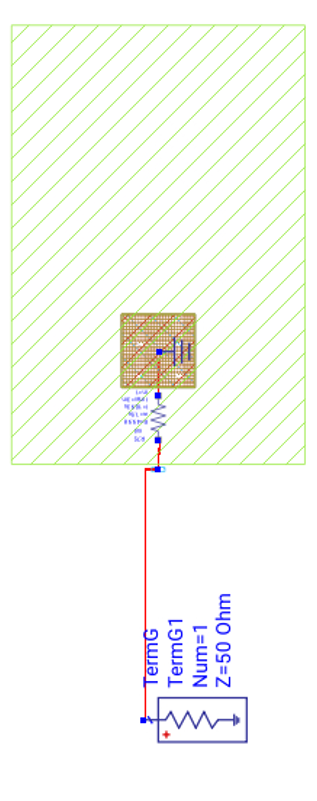
\includegraphics[width=0.3\linewidth]{Design_figures/Layout/LayoutComponents/SchematicComponents/Layout50ohmTermination_LoadComponent.png}
    \caption{Layout and schematic of the \SI{50}{\ohm} EM termination}
    \label{fig:placeholder}
\end{figure}
\end{comment}
\begin{figure}[!ht]
    \centering
    \begin{subfigure}[c]{0.3\linewidth}
        \centering
        \hspace*{-2cm}
        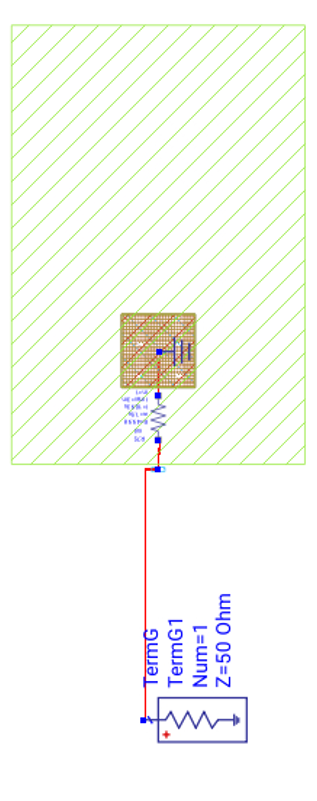
\includegraphics[width=0.6\linewidth, angle=-90]{Design_figures/Layout/LayoutComponents/SchematicComponents/Layout50ohmTermination_LoadComponent.png}
        \caption{}
        \label{fig:termination_schematic}
    \end{subfigure}
    \hfill
    \begin{subfigure}[c]{0.7\linewidth}
        \centering
        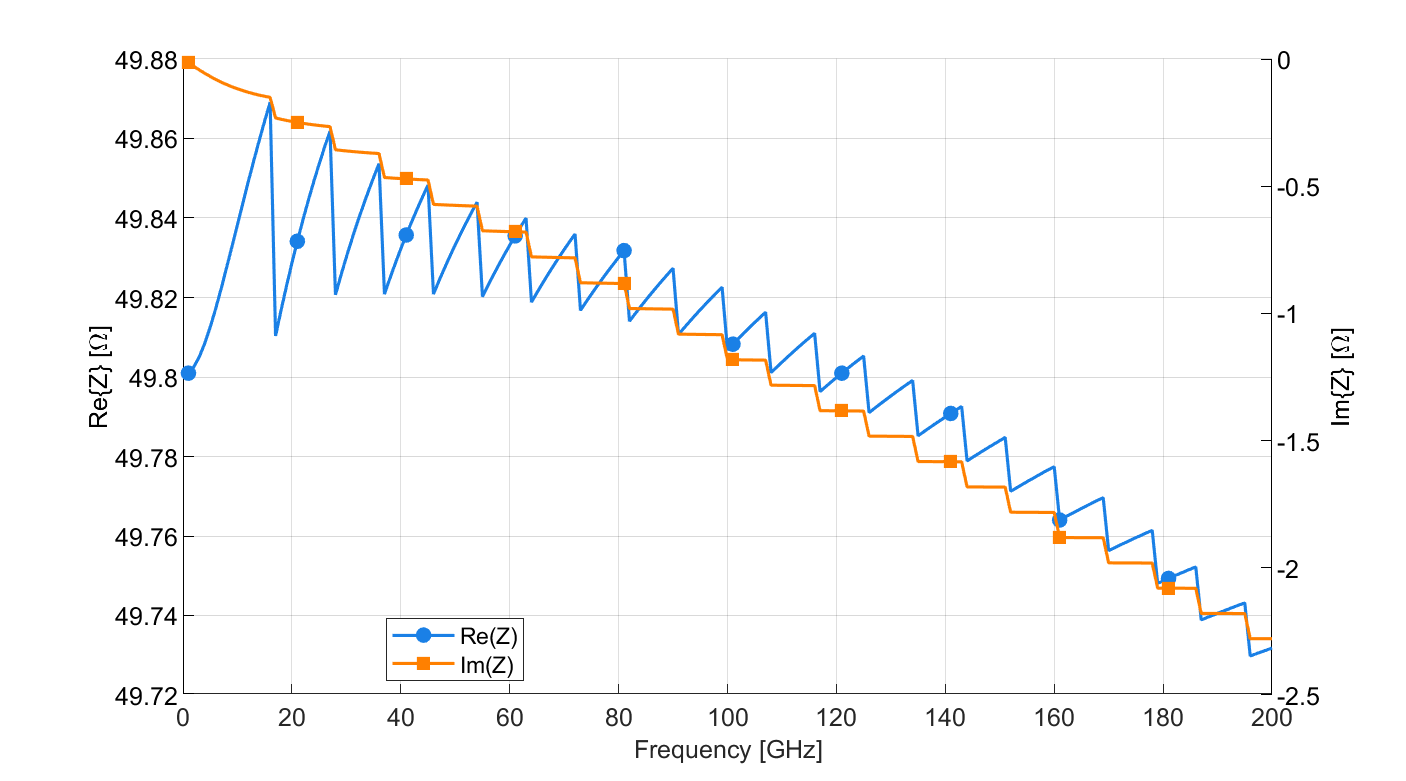
\includegraphics[width=\linewidth]{Design_figures/Layout/LayoutComponents/MeasurementsComponents/ImpedanceTermination_NormalPlot.png}
        \caption{}
        \label{fig:termination_impedance}
    \end{subfigure}

    \caption{(a) Schematic of the EM simulated \SI{50}{\ohm} termination and (b) impedance simulated in ADS and extracted from the CSV file in MATLAB.}
    \label{fig:EM_load_Terminations}
\end{figure}

\begin{landscape}

\begin{figure}[p]
    \centering
    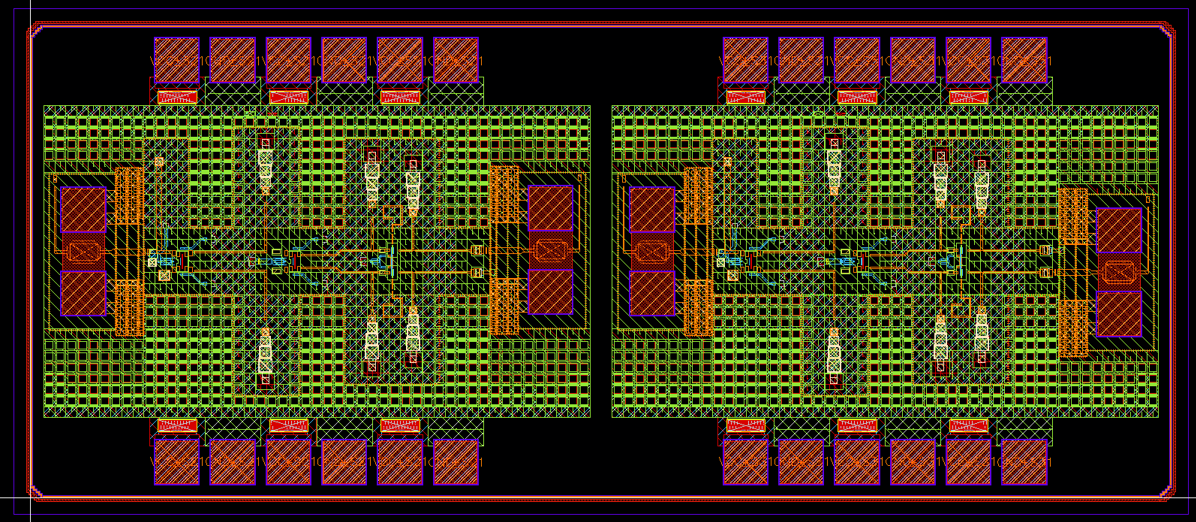
\includegraphics[width=\linewidth]{Design_figures/TapeoutChip.png}
    \caption{Chip submitted for the tapeout}
    \label{fig:TapeoutChip}
\end{figure}

\end{landscape}